\section{Algorithmic Phases and Experiment Results}

This section presents the methodology and results from a series of experiments conducted to determine the optimal combinations of algorithms for different phases of the optimization process.




\subsection{Phase 1: Hybrid Algorithmic Approach}
% Phase 1 content to be added later.

\subsection{Phase 2: Scheduling with Evolutionary Algorithm (EA)}
Once clusters have been formed in Phase 1, the next critical step is to generate a feasible schedule that defines which shops should be visited on each day of the planning period (either a single day or a custom range, as selected by the user). The primary objective during scheduling is to balance the workload across both the available days and all assigned orderbookers. This ensures that no orderbooker is disproportionately burdened and that their daily tasks are distributed as evenly as possible.

To identify the most effective scheduling strategy, a series of experiments were conducted using various algorithms. Each algorithm was evaluated based on its ability to generate balanced, constraint-compliant schedules. At the core of this evaluation process is the fitness function.

The fitness function plays a vital role in determining how practical and efficient a schedule is. It computes a cost value for each candidate schedule—lower values indicate better solutions. Hard constraints are applied first: for example, if the total route time on any day exceeds a predefined daily limit (e.g., 480 minutes), a substantial penalty is applied to immediately discourage infeasible schedules. It also checks for visit mismatches—stores not visited the required number of times—penalizing any deviations.

Additionally, soft constraints are incorporated to further refine the schedule. These include a day-balancing penalty when daily route times fall outside the ideal range (e.g., 360–420 minutes), and a geographical penalty when neighboring stores requiring only one visit are assigned to different days. These constraints collectively guide the algorithm toward generating schedules that are not only valid but also optimized for balance, practicality, and real-world efficiency. The following scheduling algorithms were used:

\begin{itemize}
    \item Simulated Annealing
    \item Ant Colony Optimization (ACO)
    \item Mixed Integer Linear Programming (MILP)
    \item Evolutionary Algorithm (EA)
\end{itemize}

Through a series of experiments, the best combination for the scheduling phase was determined, which was Evolutionary Algorithm (EA) for scheduling.
Algorithms like ACO showed that the in serach for the optimal schedule, it can often get trapped in a local optima. For MILP and simulated annealing, 
generating a schedule can be computationally expensive and time consuming. On the other hand, EA showed optmial results with genetic diversity maintained that
avoids premature convergence, hence EA is the best choice for scheduling.

\subsection{Phase 3: Route Optimization with Ant Colony Optimization (ACO)}
After a schedule has been created, the next step is to optimize the routes for each orderbooker. This involves determining the most efficient path for each orderbooker to follow, ensuring that they can visit all assigned stores in the shortest possible time while adhering to any constraints (e.g., time windows, vehicle capacity). The goal is to minimize travel distance and time while maximizing efficiency.
This phase is crucial for ensuring that the orderbookers can complete their routes within the allocated time and resources, ultimately leading to improved service levels and reduced operational costs.
Moreover, it helps determine the order of visiting the stores and the best route to take, considering factors such as road networks and other logistical constraints.
For route optimization, several algorithms were tested to identify the most effective one. The route optimization algorithms evaluated were:

\begin{itemize}
    \item Particle Swarm Optimization (PSO)
    \item Ant Colony Optimization (ACO)
    \item Google Optimization Tools (OR-Tools)
    \item Evolutionary Algorithm (EA)
    \item Dynamic Programming
\end{itemize}

It was found that the Ant Colony Optimization (ACO) route optimizer performed the best across all tested route optimization algorithms.
While POS lead to explorative results, it would often get trapped in local optimas and not perform up to the optimal mark. Using Google OR-Tools and 
Dynamic Programming showed that performance would degrade due to the very large datasets and complex constraints involved. Whereas ACO's 
pheromone mechanisms lef to effective exploration of the solution space, allowing high-quality route optimization solutions in a reasonable time frame.
\subsection{Experiments Overview}
A series of experiments were conducted across different distributors with varying numbers of stores and orderbookers. The following distributors were involved in the experiments:
\begin{table}[h!]
\centering
\begin{tabular}{|c|c|c|}
\hline
\textbf{Distributor ID} & \textbf{Number of Stores} & \textbf{Number of Orderbookers} \\
\hline
1 & 395 & 2 \\
6 & 426 & 4 \\
7 & 580 & 5 \\
131 & 42 & 1 \\
\hline
\end{tabular}
\caption{Distributors and their Assigned Stores and Orderbookers}
\end{table}

The purpose of the experiments was to determine the best combinations of scheduling and route optimization algorithms for each distributor. The experiments were designed to evaluate the performance of different algorithmic combinations in terms of distance and travel time minimization.
This was done by analyzing the total distance minimized across all orderbookers (results show average of all distributors), and the stores serviced distribution per orderbooker for each day.

\begin{figure}[H]
    \centering
    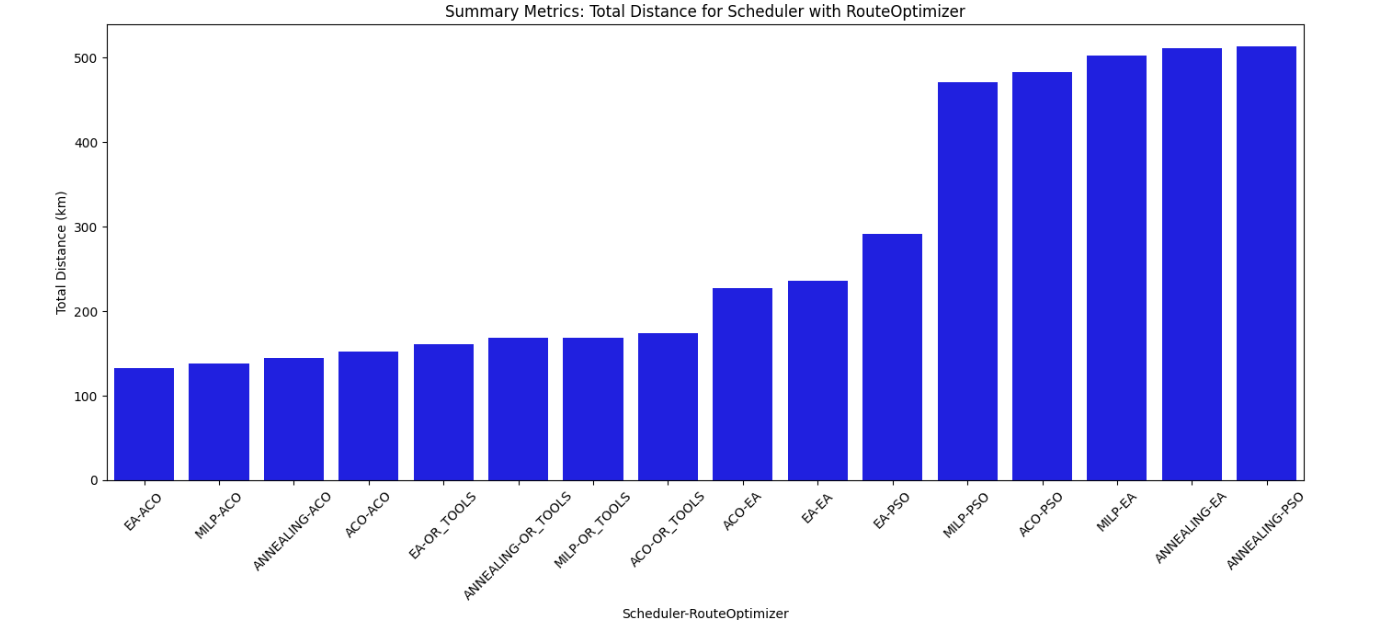
\includegraphics[width=0.95\textwidth]{images/results_distance_all_dis}
    \caption{Total distance for all distributors compared over different combinations.}
    \label{fig:results_distance_all_dis}
\end{figure}

The results in Figure~\ref{fig:results_distance_all_dis} show that the best scheduler-route optimizer combination was EA-ACO, minimizing the distance travelled to as less as 150 km as compared to almost 500 kms for the worst combination. 
It can be observed that ACO is the top 4 best route optimizers, whereas the least optimal performance was showed EA nad PSO route optimizers, and MILP and simulated annealing schedulers.


\subsection{Experiment Results}
The experiments were conducted by combining different scheduling algorithms with different route optimization algorithms. The findings of each graph is summarized below.



The best performing scheduler-route optimizer combinations for each distributor are as follows:

\begin{table}[h!]
\centering
% \begin{tabular}{|c|c|c|c|c|}
% \hline
% \textbf{Distributor} & \textbf{Orderbooker Count} & \textbf{Stores} & \textbf{Best Distance Minimized Scheduler-Route Optimizer} & \textbf{Best Travel Time Minimized Scheduler-Route Optimizer} \\
% \hline
% Distributor 7 & 5 & 580 & EA-ACO & EA-ACO \\
% Distributor 6 & 4 & 426 & EA-ACO & EA-ACO \\
% Distributor 1 & 2 & 395 & EA-ACO & EA-ACO \\
% Distributor 131 & 1 & 42 & ACO-EA & ACO-EA \\
% \hline
\begin{tabular}{|l|l|l|}
    \hline
    \textbf{Distributor} & \textbf{Best Distance Minimized Scheduler-Route Optimizer} & \textbf{Best Travel Time Minimized Scheduler-Route Optimizer} \\
    \hline
    Distributor 7 & EA-ACO & EA-ACO \\
    Distributor 6 & EA-ACO & EA-ACO \\
    Distributor 1 & EA-ACO & EA-ACO \\
    Distributor 131 & ACO-EA & ACO-EA \\
    \hline
    
\end{tabular}
\caption{Best Scheduler-Route Optimizer Combinations for Each Distributor}
\end{table}

\subsection{Conclusion}
Based on the results from the experiments, the combination of Evolutionary Algorithm (EA) for scheduling and Ant Colony Optimization (ACO) for route optimization proved to be the best-performing solution, as evidenced by its consistent performance across all distributors, particularly in minimizing both distance and travel time.

The ACO route optimizer, in particular, outperformed all other route optimization algorithms across the experiments. For distributor 131, however, the ACO-EA combination was identified as the best solution. This highlights the importance of considering both the scheduling and route optimization algorithms in tandem when evaluating their overall performance in real-world scenarios.

